\documentclass[10pt, journal]{IEEEtran}

\usepackage[T1]{fontenc} % optional
\usepackage{cite}
\usepackage{url}
\usepackage{listings}
\usepackage[usenames]{xcolor}
\usepackage{fancyvrb}
\usepackage{graphicx}

\begin{document}
\title{Economies at a Glance - A Visualisation System}
\author{
\IEEEauthorblockN{Aden Kenny - 300334300}
}
\maketitle

\section{Introduction}
~\\
For the SWEN 422 course we were given a project to develop an information visualisation system. We were given relatively free rein over the dataset we chose, so long as it was related to one of the UN Millennium Sustainable Development Goals \cite{devgoals}. We chose the development goal of "Decent Work and Economic Growth" \cite{dec}. 

This goal relates to the health of the global economy and its ability to provide enough well paying jobs for everyone that wants to work. Therefore we decided to create an information visualisation system that allows anyone to gain a basic understanding of the health of the economy of any country, and how "good" the job opportunities in that country are.



\section{System Design}

Our dataset was scraped from the CIA World Factbook \cite{cia}, and the data provides an overall view of the economies of all the countries around the world, and various economic indicators. We chose this dataset as it allows the comparison of economies as a whole, which we considered to be the best proxy for overall "goodness" of work.

The dataset was downloaded as JSON and then the relevant information was extracted and cleaned up with a Python script. This allowed us to reduce the dataset size from 13.7MB to 220KB, mainly by removing data that was not relevant to our chosen development goal.

The system was created using TypeScript \cite{ts}, React \cite{react}, and D3.js \cite{d3}. This is a fairly standard combination for web development of visualisation systems, and this stack provided a nice blend of features, and ease of use. The system was designed to be a visualisation system and it was decided that a world map or chloropleth would be the main visualisation technique used by this project. DataMaps \cite{dms}, a D3.js library was chosen to provide the chloropleth.

The system, at a high level, consists of two main parts, the "data scraper" and the "visualisation system". The data scraper is a Python script that takes a JSON that consists of data scraped from the CIA World Factbook \cite{cia}. The script then cleans this data by removing parts of the data that are irrelevant to the system, i.e. non-economic data. The overall purpose of this part of the system was to prepare the data for the main part of the system, the visualisation system. The data was then stored in a Firebase \cite{firebase} database where it was queried by the visualisation system when needed. This provided a fairly simple separation of concerns between the data and the visualisation system.

The visualisation system formed the bulk of the project, with the majority of time and resources over the course of the project being spent on it. The visualisation system itself consisted of two main parts, the first being the previously mentioned world map (or chloropleth) view, and the second being a "graph view", that was based around a bar graph. 

Both views have a navigation bar at the top of the screen which allows the user to switch between views, switch the selected economic indicator, and to show a help menu. This navigation bar stays at the top of the application as we felt that it is always useful to the user.

\subsection{Map View}

It was decided that the map view would be the main screen, the screen that a user would first see when they used the system. This was decided because the world map gives a good overview of the data, and is a good starting place for a user to view the information that the system presents and therefore is built around. The user can zoom in and out, and pan the map using the control panel to the left of the world map.

The world map view has, as the name suggests, a world map at the centre of it. The countries on the world map are coloured in relation to their selected indicator value. This provides a colour gradient based on the indicators, and there are seven possible colours that a country can be shaded. The colours range from light yellow to brown. In order to get values for the shading, the range between the minimum and maximum values is calculated and then the range is split into seven equal parts. Each country, based on the selected indicator value, is then assigned a colour from the range. This colouring allows a user to quickly view the world map and gain a basic overview of the countries based on the selected indicator. This ability to quickly glance at an economy was a key goal that occurred frequently in our scenarios. This meant that we placed a significant amount of emphasis on the importance of the map view, and resources were allocated as such.

The world map view also presents the advantage of being able to clearly communicate the relationship between countries based on economic indicators. This is especially apparent when countries fall into the same indicator range (one of the seven splits). In this case the countries will be shaded with the same colour and a relationship is strongly suggested. The shown relationships are also dynamic due to the ability of the user to change the economic indicator that is being displayed.

If a user wants to view more in depth information about a country, they can click on the country on the map and a panel is brought up to the right of the map. This panel lists all available economic indicators, not just the selected indicator. This allows the user to gain a detailed view of an individual economy, and it was a major goal that was listed in our scenarios. The alternative to the design decision of having all the indicators shown in the side menu would be to have only the currently displayed indicator on the side menu. This has two major downsides, firstly, this would mean that the system would not display an overall view of an economy at all. Secondly, the alternative is partially fulfilled in the graph view portion of the software.

\subsection{Graph View}

The second main view is the graph view. It is designed for a more in depth comparison of indicators across countries. The map view has some weaknesses when showing indicators that have data points that are major outliers, as many countries will be the exact same shade, which makes drawing any conclusions from the visualisation difficult. The graph view is designed to help to mitigate this issue. Some indicators that are available in the map view are not available in the graph view as they do not make sense shown in a bar graph style. Examples of this include indicators based on rank (e.g. Venezuela having the lowest 223th lowest growth rate in 2017), as it makes little sense to plot this on a bar graph. 

The graph view has a side panel to the right. This panel includes the country select menu. This menu allows a user to select countries that they want to be displayed on the graph. The countries are, in the default view, grouped by region, and the user can click on any of the regions and each country in the region will be selected to be shown on the graph. The region groups can also be expanded so the user can select individual countries. Additionally, there is a search bar, and this means that the user can search specific countries individually to add to the comparison list. A user can add any number of countries to the comparison list, but adding 150 countries will probably diminish the usefulness of the graph, as would adding just one.

Once the user has selected a set of countries to show on the graph they can select an indicator they wish to be graphed. A graph is then drawn from the data, from the selected set of countries, for the selected indicator. The bars on the graph can be hovered over, and it will pop up with the exact value for that country, which helps the user to get more exact data, rather than being constrained with the graph.

\begin{figure}[h]
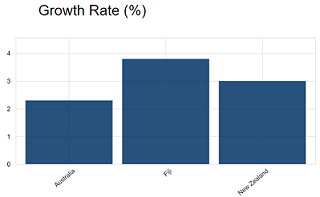
\includegraphics{graph.png}
\caption{A screenshot of the graph view showing growth rate versus country, with Australia, Fiji, and New Zealand being the selected countries}
\end{figure}
 
\section{System Justification}

\section{Contributions}

\section{Evaluation}

\subsection{Evaluation - Description}

\subsection{Evaluation - Interpretation}

\section{Evaluation Improvements}

\section{Conclusion}


\nocite{*}
\bibliographystyle{ieeetr}

\bibliography{bibliography}
\end{document}